% Generated from checked result files.
\subsection{Frozen final transfer evaluation}
\begin{table}[H]
\caption{Final TUM L256: clip scale--shift alignment, source pixel-pooled. AbsRel, RMSE and TCE lower is better; $\delta_1$ higher is better. Fail is the number of clips with any invalid fitted disparity; failures remain in aggregates.}\label{tab:final256}
\centering\small
\begin{tabular}{lrrrrr}\toprule
Model & AbsRel & RMSE & $\delta_1$ & TCE & Fail \\
\midrule
Sparse K30 & 0.1869 & 1.3742 & 0.7382 & 0.0352 & 0/13 \\
Sparse K5 & 0.1828 & 1.3531 & 0.7468 & 0.0357 & 0/13 \\
Dense carry & 0.1837 & 1.3488 & 0.7465 & 0.0328 & 0/13 \\
Dense reset & 0.1909 & 1.3778 & 0.7412 & 0.0348 & 0/13 \\
Output hold & 0.1955 & 1.3877 & 0.7332 & 0.0345 & 0/13 \\
DA2 Small 252 & 0.2166 & 2.1519 & 0.6686 & 0.0709 & 2/13 \\
MiDaS Small 256 & 0.1849 & 1.3476 & 0.7369 & 0.0640 & 0/13 \\
DPT-Large 256 & 0.1894 & 1.3559 & 0.7201 & 0.0690 & 0/13 \\
\bottomrule\end{tabular}
\end{table}
\begin{table}[H]
\caption{Final TUM L8: clip scale--shift alignment, source pixel-pooled. AbsRel, RMSE and TCE lower is better; $\delta_1$ higher is better. Fail is the number of clips with any invalid fitted disparity; failures remain in aggregates.}\label{tab:final8}
\centering\small
\begin{tabular}{lrrrrr}\toprule
Model & AbsRel & RMSE & $\delta_1$ & TCE & Fail \\
\midrule
Sparse K30 & 0.1840 & 10.1931 & 0.8017 & 0.0578 & 7/462 \\
Sparse K5 & 0.1837 & 10.1759 & 0.8032 & 0.0590 & 6/462 \\
Dense carry & 0.1946 & 10.9170 & 0.8020 & 0.0572 & 7/462 \\
Dense reset & 0.1669 & 8.6731 & 0.7979 & 0.0503 & 8/462 \\
Output hold & 0.1677 & 8.5613 & 0.7965 & 0.0484 & 8/462 \\
DA2 Small 252 & 0.2074 & 16.9349 & 0.8305 & 0.1285 & 45/462 \\
MiDaS Small 256 & 0.1539 & 9.5211 & 0.8270 & 0.0716 & 22/462 \\
DPT-Large 256 & 0.1810 & 10.4890 & 0.8402 & 0.1004 & 9/462 \\
\bottomrule\end{tabular}
\end{table}
These panels measure aligned relative shape, not calibration-free metric depth. The selected K30 model is retained irrespective of its test ranking. All 13 L256 and 462 L8 clips were processed; 0 clips had no scorable GT.
\begin{table}[H]
\caption{Final L256 native K30: alignment gauges must not be conflated.}\label{tab:gauges}
\centering\small
\begin{tabular}{lrrrr}\toprule
Gauge & AbsRel & RMSE & $\delta_1$ & TCE \\
\midrule
none & 0.2014 & 1.3372 & 0.7553 & 0.0468 \\
median & 0.2094 & 1.3231 & 0.7416 & 0.0480 \\
scaleshift & 0.1869 & 1.3742 & 0.7382 & 0.0352 \\
\bottomrule\end{tabular}
\end{table}
\begin{table}[H]
\caption{Exploratory equal-sequence L256 AbsRel differences (K30 minus comparator), $n=4$. Unadjusted percentile sequence-bootstrap intervals; exact sign flips.}\label{tab:paired}
\centering\small
\begin{tabular}{lrrr}\toprule
Comparator & Difference & 95\% interval & $p$ \\
\midrule
Dense carry & +0.0023 & [-0.0052, +0.0094] & 0.625 \\
Sparse K5 & +0.0035 & [-0.0007, +0.0082] & 0.375 \\
MiDaS Small 256 & +0.0054 & [-0.0292, +0.0359] & 0.625 \\
DPT-Large 256 & +0.0011 & [-0.0398, +0.0430] & 0.750 \\
\bottomrule\end{tabular}
\end{table}
\subsection{Development diagnostics and pipeline cost}
Across 1024 development frames, all 32 post-initial keyframes have zero same-state local defect. Nevertheless, the median concatenated hidden/cache state RMS differences at those keyframes are 0.932, 0.490, 0.721, 1.069 in manifest sequence order. These are internal-state units, not depth errors. Cache age never exceeds 29. The FP64 first-block shared-input shadow bound holds at all 1024 steps; this does not certify FP32 end-to-end error. Full sequence names and frame traces are in the supplement.
On the four matched development clips, sparse K30 takes 7.496 ms/frame versus 7.521 for dense carry, a 0.33\% reduction. MiDaS Small takes 9.439 ms with matched-subset AbsRel 0.1637 versus 0.1630 for K30. That operating-point comparison is not statistical equivalence: on all 13 development L256 clips, K30/MiDaS AbsRel is 0.2091/0.1749. The native sparse stream uses 13.501 MiB of persistent state versus 12.000 MiB dense. Read/decode/preprocessing accounts for 69.4\% of a separate synchronized profile. The associated idealized fixed-input ceiling is 1.44 times that profile, not a measured speedup.
Existing final-stage seed replicates give source-balanced scale--shift AbsRel $0.1146\pm0.0007$ on development L8 and $0.2040\pm0.0077$ on development L256 (mean and sample SD, three seeds sharing the earlier training stages).
\begin{figure}[H]
\centering
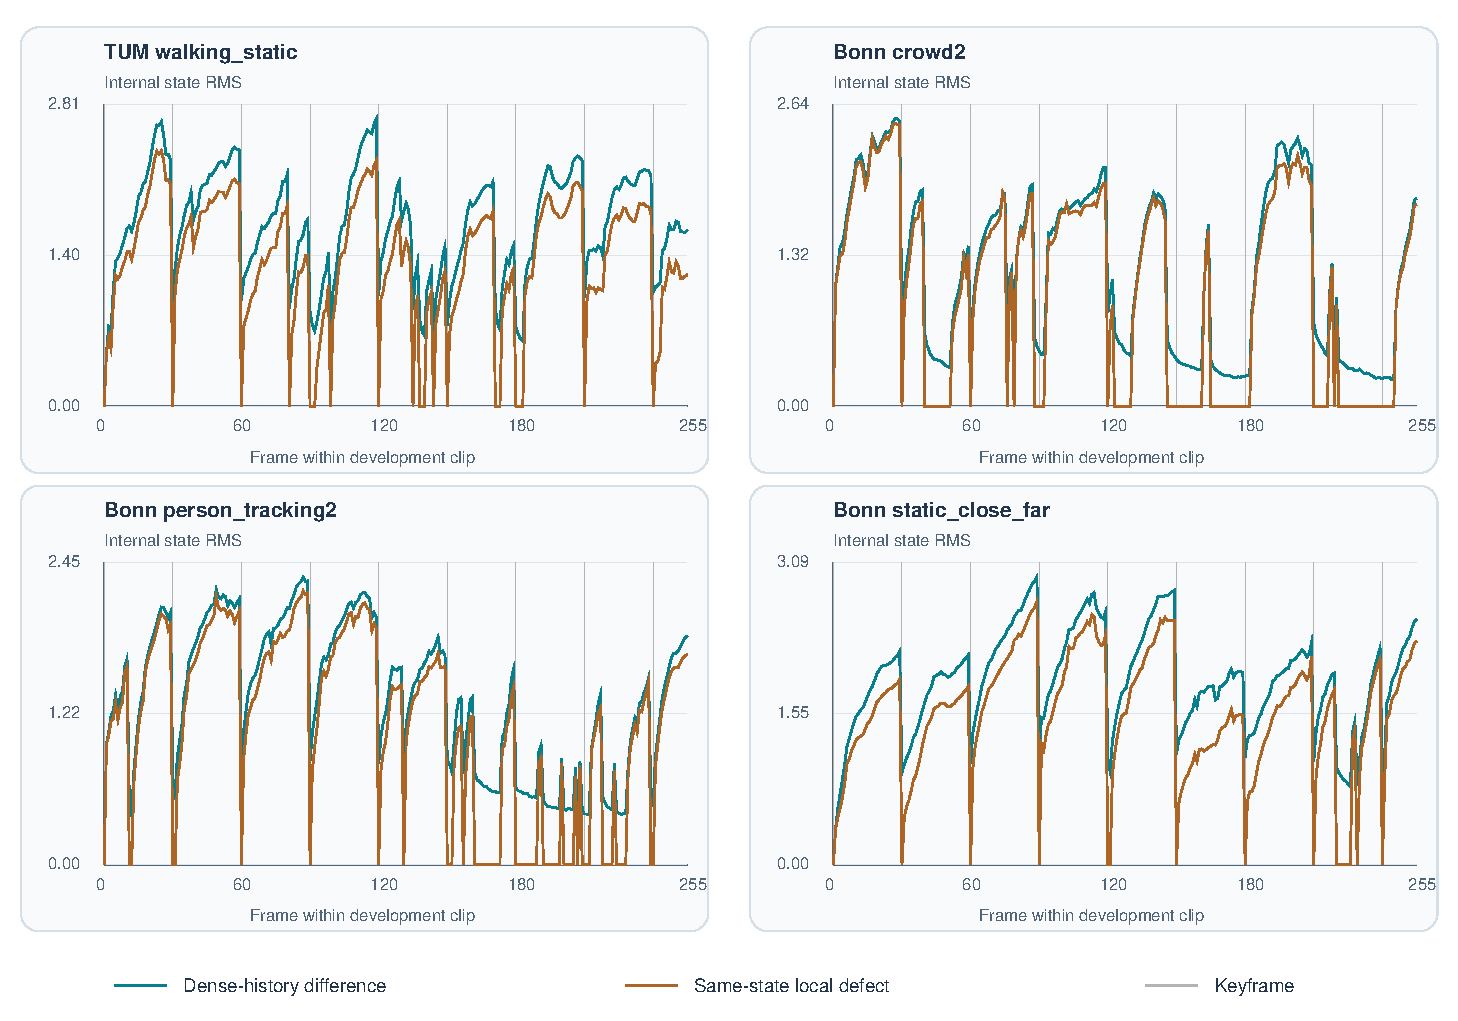
\includegraphics[width=\linewidth]{figures/development_state_diagnostic.pdf}
\caption{Development-only extended-state diagnostics. Dotted lines mark keyframes. The same-state local defect vanishes at refresh, while the difference from the separately evolved dense history persists. Curves are RMS over concatenated hidden states and caches, not GT depth error or uniquely allocated memory.}\label{fig:diagnostic}
\end{figure}
